\documentclass[11pt]{article}
\usepackage[T1]{fontenc}
\usepackage[utf8]{inputenc}
\usepackage{lmodern,microtype}
\usepackage[margin=1in,headheight=15pt]{geometry}
\usepackage{amsmath,amssymb,amsthm,mathtools}
\usepackage{booktabs,array,longtable,enumitem,needspace}
\usepackage{graphicx,xcolor,hyperref,xurl,fancyhdr,listings,tikz}
\usetikzlibrary{arrows.meta,positioning,fit}
\definecolor{ink}{RGB}{28,57,77}
\definecolor{accent}{RGB}{20,112,124}
\definecolor{pale}{RGB}{243,247,248}
\hypersetup{colorlinks=true,linkcolor=ink,citecolor=ink,urlcolor=accent,
 pdftitle={Lazy Weight Replay and Native Chamber Graphs for Unknot Recognition},
 pdfauthor={Research continuation for Vladimir Reshetnikov's ProveIt project}}
\pagestyle{fancy}\fancyhf{}
\fancyhead[L]{\small Lazy replay and native chamber graphs}
\fancyhead[R]{\small ProveIt research continuation}
\fancyfoot[C]{\thepage}
\setlength{\parskip}{0.35em}
\setlength{\parindent}{1.1em}
\setlength{\emergencystretch}{3em}
\newcolumntype{L}[1]{>{\raggedright\arraybackslash}p{#1}}
\setlist{itemsep=0.25em,topsep=0.4em}
\lstset{basicstyle=\ttfamily\footnotesize,breaklines=true,columns=fullflexible,
 showstringspaces=false,frame=single,framerule=0.25pt,
 backgroundcolor=\color{pale},xleftmargin=0.35em,xrightmargin=0.35em}
\newtheorem{theorem}{Theorem}[section]
\newtheorem{lemma}[theorem]{Lemma}
\newtheorem{proposition}[theorem]{Proposition}
\newtheorem{corollary}[theorem]{Corollary}
\theoremstyle{definition}
\newtheorem{definition}[theorem]{Definition}
\newtheorem{example}[theorem]{Example}
\newtheorem{remark}[theorem]{Remark}
\newcommand{\Z}{\mathbb Z}
\newcommand{\Q}{\mathbb Q}
\newcommand{\poly}{\operatorname{poly}}
\newcommand{\bits}{\operatorname{bits}}
\newcommand{\cc}{\operatorname{cc}}
\newcommand{\rank}{\operatorname{rank}}
\newcommand{\cut}{\mathbin{\backslash\!\backslash}}
\DeclareRobustCommand{\code}[1]{\nolinkurl{#1}}
\newcommand{\Run}{\mathcal R}
\newcommand{\Cost}{\mathcal C}
\newcommand{\BaseCommit}{\texttt{e0b2f802f336fcb51e9ec5f29174cfe28dfb9d39}}
\begin{document}
\hypersetup{pageanchor=false}
\begin{titlepage}
\vspace*{0.28in}
{\large\sffamily\color{accent} TOPOLOGY / COMPUTATIONAL GEOMETRY\par}
\vspace{0.25in}
{\LARGE\bfseries Lazy Weight Replay and\par Native Chamber Graphs\par}
\vspace{0.16in}
{\Large for Unknot Recognition\par}
\vspace{0.25in}
{\large Receiver-independent interval transport,\par
source-authenticated nonseparating batches,\par
and a reproducible implementation\par}
\vspace{0.28in}
{Research continuation prepared for Vladimir Reshetnikov's ProveIt project\par}
{Developed with ChatGPT; 12 October 2026\par}
\vspace{0.2in}
\begin{abstract}
Two concrete operations remain costly or incomplete in the current compressed
geometry program. The weighted certificate checker repeatedly reconstructs
constant-run partitions, including receiver intervals on which the same
vector is added uniformly. The earlier chamber-graph framework, meanwhile,
accepts geometric component labels and side locations that its native caller
does not yet supply.

We replace the checker's flat weight state by a deterministic balanced
sequence with implicit integer lengths and lazy vector additions. A
translation or reflection fold with \(S\) deleted suffix runs uses
\(O((S+1)\log(R+2))\) tree work, together with residue sorting for translations,
independently of the number of receiver runs. A complete family of legal
Agol--Hass--Thurston traces separates the previous \(\Omega(HL)\) repeated
receiver work from the new \(O(L+H\log(L+2))\) weight transport. We retain the
independent residue-derivative arithmetic and the original certificate schema.

We also implement a native chamber-graph exporter for a supplied normal
surface with explicit component representatives. Exact scalar orbit censuses
authenticate the component labels and locate both sides in the cut
complement; the normal double checks two-sidedness. An independent checker
reconstructs the side markers from raw cut-cell charts. The resulting graph
supports the earlier exact cographic criterion for simultaneous
nonseparation on actual source inputs.

The package contains complete proofs, code, independent checks, source
fixtures, certificates, paired measurements, and integration instructions.
Classical weighted orbit counting, the previously proved two-boundary run
bound, and the earlier cographic theorem are explicitly attributed. The
remaining hierarchy-discovery, witness-transport, restart, and encoded-state
obligations are not assumed solved. No general quasi-polynomial unknot
recognition theorem is claimed.
\end{abstract}
\vfill
{\small\textbf{Source checkpoint.} \BaseCommit.\par
\textbf{Status.} Local algorithms and their stated bounds are proved;
finite experiments test the delivered implementation. The global
\(n^{O(\log n)}\) target remains open for this implementation.}
\end{titlepage}
\pagenumbering{roman}
\hypersetup{pageanchor=true}
\begingroup
\setlength{\parskip}{0pt}
\small
\tableofcontents
\endgroup
\clearpage
\pagenumbering{arabic}
\section{Purpose, checkpoint, and contribution}
\label{sec:scope}

The aim of this continuation is to improve operations that an eventual
efficient geometric recognizer must execute, while making their mathematical
and implementation contracts precise. The result has two parts. The first
accelerates an existing independently checked operation. The second supplies
a missing geometric input to an earlier graph algorithm. Their relationship
is direct: the new geometric observer is itself built from weighted orbit
queries, so it benefits from improved weighted replay without weakening the
source checks.

\subsection{The present complexity target}

Lackenby's February 2021 announcement states an
\(n^{O(\log n)}\) unknot recognition bound in the crossing number
\cite{announcement,talk}. His July 2026 preprint gives a hierarchy algorithm
for incompressibility and unknot recognition. Section~9 explicitly leaves
some operation costs insufficiently specified for a time estimate.
Proposition~9.1 gives the iteration bound \(L(g+1)^L\);
Proposition~10.2 bounds refined hierarchy length by
\(4c_q(\mathcal H)\). Theorems~14.1 and 14.4 provide efficient hierarchy
encoding and compressed cutting results \cite{lackenby26}. These are
substantial existing results. This paper neither reconstructs a complete
proof of the announced bound nor attributes a new polynomial weighted-orbit
theorem to itself.

Classical Agol--Hass--Thurston orbit counting and its weighted extension are
the mathematical foundation of the local operations studied here
\cite[Theorems~12 and 16]{aht}. The question addressed by our first part is
more specific: how much of the current weight partition must an independently
checked replay actually revisit?

\subsection{Encoding and notation}

The global target uses the diagram crossing number \(n\). For a local
normal-surface query, \(T\) is the tetrahedron count, \(B\) the maximum
normal-coordinate bit length, and \(k\) the number of explicitly labelled
components. For an orbit query, \(N\) is the numerical interval size,
\(R\) the number of canonical constant runs, and \(d\) the dimension of a
weight vector. Endpoint costs depend on \(\log(N+1)\), not on \(N\)
literal iterations. A certificate is itself input to its checker, so its
encoded length is charged whenever an arbitrary supplied trace is
considered. These distinctions prevent an operation count in a large
normal coordinate from being mistaken for a polynomial encoded bound.

\subsection{What was inspected}

The implementation checkpoint is \BaseCommit, the \code{main} revision
observed at the beginning of this work. All patches and reproduced
measurements in the package refer to that fixed source. Later repository
changes are not silently incorporated into the baseline.

The inspected source includes the native \code{fastunknot} modules for
weighted histograms, weighted representative transversals, normal surface
geometry, raw cut cells, cut complement components, parallelity bundles,
ordered boundary interfaces, and supplied-cut handlebody certification. The
maintained source and reports distinguish these supplied geometric queries
from the complete diagram recognizer \cite{repo}.

The incoming directory at this checkpoint contains four relevant packages:
\emph{Exceptional Rows}, \emph{Matroidal Dual Forests},
\emph{Nonlinear Activation Forests}, and \emph{Ordered Interface Kernels}.
Their source and integration descriptions were inspected for overlap.
They address finite forest/cancellation selection and related replay
optimizations. None supplies the lazy receiver operation or the native
component-labelled chamber exporter delivered here. Earlier reports do,
however, prove several tempting candidate results already. These
are used with attribution.

\begin{table}[htbp]
\centering\small
\begin{tabular}{L{0.24\textwidth}L{0.34\textwidth}L{0.32\textwidth}}
\toprule
Topic & Earlier result & Contribution of this continuation\\
\midrule
Weighted orbit counting &
Polynomial encoded computation, classical AHT &
A faster replay of the same checked traces\\
\addlinespace
Native fold run growth &
\(R_T\le R_0+2T\), already in \code{suffix_folds.tex} &
Use this bound to control a lazy balanced representation\\
\addlinespace
Receiver-local arithmetic &
Flat producer work \(O(R)+O((S+P)d)\) &
Remove the receiver-run term \(P\) from tree and vector updates\\
\addlinespace
Chamber graphs &
One-census compiler and cographic nonseparation in report~92 &
Authenticate labels and side locations from actual normal coordinates\\
\addlinespace
Hierarchy resets &
Weighted dependency-path bounds in reports~23 and~92 &
No replacement theorem asserted; identify the still-missing geometric bridge\\
\bottomrule
\end{tabular}
\caption{Attribution and scope. \(R\) is the total number of weight runs,
\(S\) the deleted suffix runs, \(P\) the receiver runs, and \(d\) the vector
dimension.}
\label{tab:scope}
\end{table}

\subsection{The first main result}

The earlier suffix-fold optimization already avoids some vector additions
outside the receiving interval, but its state is a flat sequence
\cite{suffix}. A receiver containing many different vectors is still
visited throughout. The checker reconstructs even more of the flat
partition. This is a representation cost, not a necessary part of checking
the topological source.

Our key observation is elementary but useful: adding the same vector to all
runs of an interval preserves every equality and inequality between
neighbouring runs inside that interval. An exact checker can therefore
store that addition at the root of a balanced subtree. It need only split
at the interval endpoints and inspect the two resulting seams.

Theorem~\ref{thm:lazy-fold} makes this observation quantitative. In
particular, the work does not grow with the number of pre-existing receiver
runs. The complete source family in Theorem~\ref{thm:star} shows why this
changes an asymptotic term rather than only a constant factor. The
implementation preserves the residue-anchor and discrete-derivative
checker, so production and replay still use different transport arithmetic.

\subsection{The second main result}

A finite graph can encode which components of a disjoint two-sided surface
system may be cut simultaneously without disconnecting the ambient manifold.
The graph alone is easy to use. The difficult interface question is whether
its vertices and edges genuinely describe the supplied source.

The native exporter takes one embedded normal surface together with an
explicit representative disc for each of its claimed connected components.
It verifies that the representatives are distinct and exhaustive
\emph{as component labels}, verifies two-sidedness, and locates both sides
of each component in the actual cut complement. A successful certificate
therefore supplies the missing geometric contract of report~92 for this
input class \cite{persistence}. Its checker derives side locations through
a separate raw cut-cell construction rather than importing the exporter.

The number of components \(k\) is an explicit input/output parameter. A
normal vector can encode an enormous number of parallel components. This
exporter does not compress an exponentially large arbitrary labelled graph
into a constant-size answer. For a connected large-coordinate surface,
however, \(k=1\), and a single representative suffices regardless of the
number of normal discs.

\subsection{What the results establish}

The local replay theorem is unconditional for the specified checked
interval trace and exact weight representation. The native chamber theorem
is unconditional under the implemented geometric source contract:
a validated finite connected compact orientable triangulation with one
torus boundary, an admissible normal vector, and correctly authenticated
component representatives whose two-sidedness gate succeeds.

The chamber theorem does not require the components to be incompressible,
and does not prove that they are. The resulting graph certifies
nonseparation only. Neither a connected complement nor a graph loop is a
handlebody certificate. Moreover, the graph does not yet contain a
geometric path crossing a particular component once, or a support
certificate showing that such a path survives a later edit.

For the same reason, the new replay engine does not alter the correctness
criterion of the complete recognizer. It reduces work needed to check
existing local certificates. A performance claim about a supplied normal
cut is reported as such, rather than as a speed-up for arbitrary knot
recognition.

\subsection{Novelty in the appropriate sense}

Balanced sequence trees, delayed range additions, normal-surface
connectivity, and dual graphs are established ideas. No priority claim is
made for those foundations. The contributions here are the exact
receiver-independent replay construction with its native trace separation,
the source-derived chamber-label interface and its independently reconstructed
checker, and the executable evidence connecting them to this implementation.
An exhaustive literature priority search for these combinations has not
been performed. The proofs should be judged on their stated claims, and the
measurements on their executed scopes.

\section{Receiver-independent evaluation of weighted orbit folds}
\label{sec:lazy-weight-theory}

The existing native suffix-fold theorem~\cite{suffix} gives
$R\le R_0+2\tau$ canonical weight runs after $\tau$ truncations,
including signed vector weights. Static contraction cannot increase this
number. The mass bound and polynomial selector accounting are also already
established in the repository~\cite{weighted}. Classical weighted orbit computation was
proved polynomial by Agol--Hass--Thurston
\cite[Lemma~15 and Theorem~16]{aht}.
Our change concerns how much of that bounded state must be visited after
one particular fold. The preceding native implementation still scans the
entire run list, and performs vector arithmetic on every receiving run.
A lazy additive run tree removes both dependencies.

\subsection{Exact lazy actions on canonical run trees}

A run is a pair $(\ell,v)$, where $\ell$ is a positive integer length and
$v\in\mathbb Z^d$. A canonical run sequence has unequal values in consecutive
runs. Its lengths sum to the current universe size. Store it in a balanced
binary tree whose leaves are runs. Each subtree stores its leaf count,
height, total length, first value, last value, and a pending additive tag.
Heights are balanced by the number of leaves, independently of their
possibly enormous integer lengths.

\begin{lemma}[Uniform additions preserve internal run boundaries]
\label{lem:lazy-translation}
For any $u,v,z\in\mathbb Z^d$, one has $u=v$ if and only if
$u+z=v+z$. Consequently adding the same vector $z$ to every point of a
canonical subtree changes none of its internal run boundaries. It can be
represented by adding $z$ to the subtree tag and to its two endpoint
values. Canonicalization after reconnecting this subtree is required only
at the two external seams.
\end{lemma}
\begin{proof}
Subtract $z$ from the equality in either direction. The internal adjacencies
are unchanged, so every old unequal pair remains unequal. Only an adjacency
between an updated value and an unupdated value can change its equality
status, and these are precisely the external seams.
\end{proof}

The tag denotes a common increment not yet propagated to descendants.
Before a split or rotation changes a tagged node's descendants, the tag is
pushed to the current children and cleared at that node. Otherwise the scope
of the increment would change. This push rule is part of the invariant,
not an optional implementation convention.

\begin{proposition}[Run-tree primitives]
\label{prop:run-tree}
A deterministic height-balanced run tree on $R$ canonical runs supports
splitting at an arbitrary integer position, concatenation with boundary
coalescing, and adding a constant vector on a contiguous position interval
using $O(\log(R+2))$ structural operations and $O(d\log(R+2))$ integer
additions or comparisons. These operations need not inspect the other leaves
of the affected interval. Reporting or deleting $s$ specified consecutive
runs costs $O(s+\log(R+2))$ structural operations, apart from output work.
\end{proposition}
\begin{proof}
Use a leaf-oriented AVL tree, with empty-tree height zero and leaf height
one. Joining trees of heights $a,b$ takes $O(|a-b|+1)$ structural operations,
and its output height $c$ lies in
$\{\max(a,b),\max(a,b)+1\}$. Indeed, join descends the taller spine until
the two heights differ by at most one. The height gap decreases at each
descent, and each returning frame requires at most one single or double
rotation. Induction gives the stated output-height property. The minimum
number of leaves in an AVL tree satisfies the Fibonacci height recurrence,
so every height in question is $O(\log(R+2))$.

Stored subtree lengths identify the child containing a split position.
Only one root-to-leaf path is followed; if the position is inside a leaf,
that leaf becomes two positive-length runs of equal value in the two
separate output trees. Push pending tags along the path and use AVL joins
to reassemble its off-path pieces. The sum of these join costs is
logarithmic, not the product of two logarithmic bounds. To see this
explicitly, first observe inductively that each output fragment has height
at most that of the subtree being split. At a right turn on the split path,
let $a$ be the left sibling's height and $b$ the height of the left fragment
returned from the right child. The original AVL inequality gives
$b\le a+1$. The newly joined left fragment has some height $c\ge b$.
If $a\ge b$, then $a-b\le c-b$; if $b>a$, then $b-a\le1$.
Consequently this join costs $O(c-b+1)$. As the split returns toward the
root, the height of the accumulated left fragment increases only at right
turns. These height increases telescope to at most the original root
height. Left turns give the symmetric telescoping bound for the right
fragment. There are at most one root-height's worth of returning frames,
so all joins and tag pushes together take $O(\log(R+2))$ structural work.

For concatenation, compare the last realized value of the left tree with
the first realized value of the right. If unequal, use a balanced join.
If equal, remove these two extreme leaves, replace them by one leaf with
their combined length, and perform balanced joins. No new interior equality
can appear: the old neighbors of each removed leaf were unequal to its
value. Access, removal, and joining follow logarithmic-height paths.

For a range addition, split at its two endpoints, apply the tag update of
Lemma~\ref{lem:lazy-translation} to the middle tree, and concatenate the
three pieces canonically. Reporting a detached subtree visits each of its
leaves once. Empty pieces are omitted. All endpoint arithmetic is on binary
integers and never iterates over a leaf's numerical length.
\end{proof}

\subsection{Translation folds from one anchor and their jump locations}

Consider a legal native truncation from $[0,N)$ to $[0,C)$. For a positive
carrier let $p>0$ be its period and $b=C-p\ge0$. The deleted suffix is
pushed by
\[
 \rho(x)=b+((x-b)\bmod p)
\]
onto $[b,C)$. Let $f$ be the old suffix weight, extended by zero off
$[C,N)$, and define the added residue sum
\[
 F(r)=\sum_{x\equiv r\pmod p}f(x),\qquad b\le r<C.
\]
For $b<r<C$, finite summation gives
\begin{equation}\label{eq:lazy-residue-jump}
 F(r)-F(r-1)=\sum_{x\equiv r\pmod p}\bigl(f(x)-f(x-1)\bigr).
\end{equation}
One anchor determines the remaining additive constant. If the suffix
intersects $S$ constant runs $[l_j,h_j)$ with values $v_j$, then
\begin{equation}\label{eq:lazy-residue-anchor}
 F(b)=\sum_{j=1}^{S}
 \left(\left\lfloor\frac{h_j-1-b}{p}\right\rfloor
       -\left\lfloor\frac{l_j-1-b}{p}\right\rfloor\right)v_j.
\end{equation}
Only the clipped suffix run endpoints are used. Every left endpoint
contributes $+v_j$ to its residue jump and every right endpoint contributes
$-v_j$. Combine coincident locations, omit the jump at $b$ when integrating
from the anchor, and sort the remaining locations. This produces $O(S+1)$
constant addition intervals. The operations on quotient and residue values
use binary division and multiplication; they do not enumerate a residue
class or repeat a shift a numerical number of times.

\begin{theorem}[Receiver-independent native fold]
\label{thm:lazy-fold}
Suppose the old weight function has $R$ canonical runs and the deleted suffix
meets $S$ runs. A native translation fold can be evaluated exactly in
\[
 O\bigl((S+1)\log(R+2)+S\log(S+1)\bigr)
\]
structural and endpoint-order operations and
$O(d(S+1)\log(R+2))$ vector-coordinate operations, with binary integer costs
charged separately. A reflection fold obeys the same bound without the
$S\log(S+1)$ sorting term. Neither bound contains the number of receiving
runs or of untouched prefix runs. The resulting tree denotes the same
canonical function as the established native suffix-only operation.
\end{theorem}
\begin{proof}
Split off and report the deleted suffix, costing $O(S+\log(R+2))$ by
Proposition~\ref{prop:run-tree}. For translation, compute
\eqref{eq:lazy-residue-anchor} and the $O(S)$ residue events in
\eqref{eq:lazy-residue-jump}. Sorting and integrating them gives the exact
piecewise-constant function $F$ on the receiving interval. Add each nonzero
constant piece with the run-tree range-add primitive. There are $O(S+1)$
pieces, and all are inside the retained prefix. Their interiors are disjoint,
so the sum of the range updates is exactly $F$. The old prefix remains
pointwise unchanged except for the prescribed additions. Exact seam
coalescing after every update leaves a canonical result.

For reflection $x\mapsto K-x$, the image of $[l_j,h_j)$ is
$[K-h_j+1,K-l_j+1)$. These intervals occur in reverse order and remain
disjoint, so they can be reported directly in increasing image order and
added as constant ranges. No sorting of image endpoints is needed.

During successive range additions there can be temporary boundaries that
cancel only after a neighboring interval is updated. At most two boundaries
per update are introduced. Thus the transient run count is $O(R+S+1)=O(R+1)$;
using its logarithm instead of $\log(R+2)$ changes only the constant factor.
This justifies the height bound throughout the operation, not merely at its
end. The proof makes no assumption that a nonzero vector has positive
coordinates.
\end{proof}

\subsection{Full-trace cost and integer sizes}

Let a complete forward trace contain $\tau$ truncations and $E$ events in
all. For truncation $t$, let $S_t$ be its deleted suffix run count. For
contraction $j$, let $G_j$ be its number of static gaps and $D_j$ the number
of constant run pieces actually emitted. Put $R_* = R_0+2\tau$ using the
existing native run-growth theorem.

\begin{corollary}[Weighted replay ledger]
\label{cor:lazy-replay}
After canonical input preparation, the new weight evaluator requires
\[
 O\left(
 R_0+E+\sum_{t=1}^{\tau}
       \bigl((S_t+1)\log(R_*+2)+S_t\log(S_t+1)\bigr)
 +\sum_j\bigl(G_j\log(R_*+2)+D_j\bigr)
 \right)
\]
structural work, together with the corresponding exact vector arithmetic
and histogram costs. This is additional to validation and maintenance of
the unweighted pairing trace. It contains no cumulative receiver-run term
$\sum_t P_t$.
\end{corollary}
\begin{proof}
Sum Theorem~\ref{thm:lazy-fold}. For a contraction, split out each static gap,
report its runs to the histogram, remove it, and concatenate the surviving
pieces. Using position lengths rather than absolute labels automatically
closes the removed gap. Each gap costs logarithmic split/join work; reporting
costs exactly the deleted run pieces. The input tree can be built bottom-up
from its already canonical list in $O(R_0)$ work. Pairing deletion, trimming,
merger, and transmission do not change the weight function. No work for
those events is charged to the weight tree beyond the $O(E)$ event-dispatch
term. Pairing-row maintenance is charged separately.
\end{proof}

\Needspace{12\baselineskip}
For additive input intervals $[a_i,b_i)$ with vector values $v_i$, define
\[
 A=\sum_i(b_i-a_i)\lVert v_i\rVert_\infty.
\]
\begin{lemma}[Coefficient bound for delayed transfers]
\label{lem:lazy-bits}
During replay of legal native folds and contractions, each stored base
value, pending lazy tag, endpoint-value cache, and sum of inherited tags
has every coordinate bounded by $A$ in absolute value. The auxiliary
derivative and anchor arithmetic has magnitude $O(A)$. Hence replay uses
$O(1+\log(A+1))$ coefficient bits and $O(\log(N+1))$ endpoint bits, where
$N$ is the initial universe size. Input validation additionally reads all
supplied coefficient bits, including values assigned to empty intervals.
\end{lemma}
\begin{proof}
For the proof only, introduce one atom $(i,x)$ for every input-interval
occurrence $i$ and every integer $x\in[a_i,b_i)$, carrying vector $v_i$.
The sum of the atoms' infinity norms is $A$. No implementation step
constructs these atoms. The standard orbit-transport invariant partitions
them between active points and finalized orbits. A fold moves the atoms
at each deleted point to its retained image, and a contraction finalizes
the atoms at its deleted points. Thus the active allocations are disjoint.

Refine this mathematical invariant pointwise through the lazy tree.
Partition an active point's allocated atoms between its leaf's stored
base value and the pending tags along its root-to-leaf path. Each part's
vector sum equals the corresponding stored numerical value or tag.
The atom subsets attached to one constant-valued leaf or tag may differ
from point to point; their vector sums agree. Initially the complete
allocation is in the leaf base. A uniform addition transfers disjoint
atoms from the detached suffix into each receiving point; place them in
the updated tag, or in the base when the receiving subtree is a leaf.
Pushing a tag redistributes its pointwise subsets to the same children
before any child's scope changes. Splitting restricts these subsets to
the two intervals. A rotation changes only the bracketing after this
redistribution. Coalescing equal boundary leaves places each point's
current allocation in its new base. These operations preserve the
partition invariant. If a tag or addition has numerical value zero,
its zero-sum atom subset may be rebased pointwise without changing any
stored number; cancellation therefore causes no exception to the
invariant. This is auxiliary proof bookkeeping, not extra runtime work.

Every stored base, tag, inherited-tag sum, and realized endpoint cache is
therefore the sum of some subset of the input atoms, and its coordinate
magnitude is at most $A$. This also proves
$\sum_j(h_j-l_j)\lVert v_j\rVert_\infty\le A$ for the current runs.
An anchor's run multiplicity is at most its run length, so each partial
anchor sum has magnitude at most $A$. For the suffix extended by zero,
the sum of the norms of its endpoint jumps is at most
$2\sum_j\lVert v_j\rVert_\infty\le2A$. Every partial collision sum of
mapped jumps is therefore bounded by $2A$, and combining such sums with
an anchor is bounded by $3A$. All scalar multipliers in the anchor are
counts of integer points; all divisions use a strictly positive integer
period. Their operands have $O(\log(N+1))$ bits. The result follows.
\end{proof}

The fine structural bound is deterministic for the AVL transport and its
comparison sort of residue events. The delivered Python source
canonicalizer and histogram accumulator also use dictionaries. Their
map-operation counts are separate from the tree ledger: a constant-time
or average-case hash-table model must not be silently promoted to a
worst-case comparison bound. Sorting an endpoint-event list and using an
ordered histogram map or a sorted emission ledger would give deterministic
comparison bounds with the corresponding sorting factors. The delivered
code retains its established source and histogram routines.

The star-family separation below is a statement about the actual specified
flat and lazy evaluation methods. It is not a lower bound for every weighted
orbit algorithm, and it does not bound the number of topology hierarchy
states.


\section{A complete source family separating eager and lazy replay}
\label{sec:separation}


\begin{theorem}[A native AHT star family]
\label{thm:star}
For integers $H\ge1$ and even $L\ge2$, set $N=(H+1)L$ and supply the inclusive
interval pairings
\[
 g_j:[0,L-1]\longrightarrow[jL,(j+1)L-1],\qquad 1\le j\le H.
\]
Assign weights $w(x)=x\bmod2$ on $[0,L)$ and $w(x)=1$ on $[L,N)$.
The maintained forward AHT scheduler produces exactly $H$ truncations at
$HL,(H-1)L,\ldots,L$, followed by one static contraction. Each truncated
suffix meets a single weight run, while every receiving interval contains
$L$ alternating runs. Its final histogram is
\[
 \{(H,L/2),(H+1,L/2)\},
\]
where pairs denote (weight, orbit multiplicity).

The previous eager native weight evaluator performs $\Omega(HL)$ run visits
or receiving-value updates on this family. Lazy evaluation uses
$O(L+H\log(L+2))$ weight-tree structural work after canonicalization, including
final emission. In a record-cost model charging one unit per dictionary
operation, generic source canonicalization takes $O(L\log(L+2))$ work,
and the unchanged unweighted trace checker takes $O(H^2)$ pairing-row
checks. In that model complete certificate replay costs
\[
 O\bigl(L\log(L+2)+H\log(L+2)+H^2\bigr).
\]
It has an asymptotic record-work separation from the eager method, for
example $\Omega(H^3)$ eager work versus $O(H^2\log(H+2))$ lazy work and
shared overhead when $L=2H^2$. The same upper bound has a deterministic
comparison-model realization using sorted endpoint preparation; on this
family the final histogram has only two keys. This final whole-verifier
bound counts map operations in the delivered Python implementation;
it does not assert a worst-case constant cost for its hash lookups or
for arithmetic on binary integers. The preceding weight-tree bound is
deterministic without that map-cost assumption.
\end{theorem}
\begin{proof}
All blocks $[jL,(j+1)L)$ are covered by pairing domains or ranges, so no
initial static gap exists. Only $g_1$ is periodic: its period is $L$ and its
domain and range are adjacent. For $j>1$ the distance $jL$ exceeds the domain
width, so two periodic pairings can never be merged. The unique pairing
whose range ends at $N-1$ is $g_H$, and every other pairing range ends below
$HL$. None is transmitted by $g_H$. The suffix exposed for truncation is
therefore exactly $[HL,(H+1)L)$. The carrier period is $HL$, its nominal
receiving interval is $[0,HL)$, and its transported addition is one on
$[0,L)$ and zero on $[L,HL)$. Thus only the first block changes, and
$g_H$ disappears.
The same argument applies inductively with $H-1$ in place of $H$. At the end
no pairing remains and the whole residual prefix contracts.

Every removed block still has constant value one: preceding folds changed
only the first block. After $t$ folds the first block has value
$t+(x\bmod2)$, so it retains all $L$ alternating runs. Initially its final
value one coalesces with the long suffix; after the first fold there is at
most one additional run. In all cases a removed suffix intersects one run.
Every orbit is $\{r,r+L,\ldots,r+HL\}$ for a unique $0\le r<L$, proving
the histogram formula.

The former flat evaluator scans the retained prefix and visits its $L$
alternating entries at every fold; the local-overlay producer also touches
the first block's $L$ entries to add one. This gives the stated
$\Omega(HL)$ cost.
In the lazy tree, one constant vector is added to the root of the first-block
subtree at each fold, with logarithmic splits and joins and no scan of that
subtree. The final contraction scans its $L$ leaves once. Initial source
and certificate-weight checks process $O(L)$ records. The unweighted
checker visits exactly $H+(H-1)+\cdots+1=H(H+1)/2$ current pairing rows
in its truncation precondition loops. Its only gap sort occurs after the
pairing list becomes empty; the carrier is always the last list element,
so its deletion causes no row shifts. Thus no extra $\log H$ factor is
needed for this checker. Generation of the trace is a separate phase and
is not included in this replay estimate. Add initialization and the
unchanged input/trace costs to obtain the stated bound.
\end{proof}

For $H>1$ the actual transport counters on this family are
\[
 \begin{aligned}
 \text{source runs}&=H,&
 \text{receiving runs}&=HL+H-2,\\
 \text{addition intervals}&=2H-1,&
 \text{emitted runs}&=L.
 \end{aligned}
\]
The maximum canonical run count is $L+1$. For $H=1$, the receiving and
maximum counts are both $L$. These receiving counts are logical state
sizes read from cached subtree metadata, not counts of visited leaves.

This family was checked against the maintained producer and independent
weighted verifier for $(H,L)=(1,2),(3,8),(8,64),(16,256)$: the complete operation
lists, cut positions, and final histograms agree with the theorem. These
finite executions check compatibility with the current scheduler; the proof
above establishes the arbitrary-parameter family. The examples are synthetic
interval-pairing inputs, not claimed difficult knot diagrams.

\section{A native source certificate for the chamber graph}
\label{sec:chambers}

The cographic persistence proposal in repository report~92~\cite{persistence} assumes an
authenticated chamber graph. Its integration contract explicitly leaves the
native source exporter open. We now implement this interface for the
components of one supplied embedded normal surface. The new operator is
\texttt{normal\_chamber\_graph}; independent replay is
\texttt{verify\_normal\_chamber\_graph}. Both operate on the maintained finite,
connected, orientable source triangulations with one torus boundary.

This section establishes component identities before using them as graph
edges. A list of compatible normal coordinate vectors does not by itself
specify labelled disjoint representatives. Our input instead consists of one
normal vector $x$ satisfying the source matching and quadrilateral constraints,
together with one proposed representative disc
\[
 d_i=(t_i,c_i,r_i),\qquad 0\le r_i<x_{t_i,c_i},\qquad 0\le i<k,
\]
per component. The connected components of this single embedded surface
already have a common geometric realization. Exact orbit certificates verify
that the proposed labels are exhaustive and distinct.

\subsection{Authenticating the component labels}

Let $X$ be the maintained normal-arc interval system. Its points are normal
intersection points on globally oriented source edges; its orbits are the
connected components of the normal surface. For each marked disc choose one
of its normal vertices $p_i\in X$. The source chart authenticates that this
point belongs to $d_i$.

\begin{lemma}[Exhaustive labels from a scalar census]
\label{lem:component-marker-census}
Assign the weight $2^i$ to $p_i$, adding weights when marked points coincide.
The exact weighted orbit histogram equals
\[
 \bigl\{(2^i,1):0\le i<k\bigr\}
\]
if and only if the marked discs lie in distinct surface components and every
component contains a marked disc.
\end{lemma}
\begin{proof}
Each marker is assigned once. An orbit has weight equal to the sum of the
distinct marker powers belonging to it, so the sum has no binary carries.
An unmarked component contributes an orbit of weight zero. A component
containing two or more labels contributes a weight with at least two nonzero
bits. The stated histogram therefore forces one marker per component and no
unmarked component. Conversely, an exhaustive distinct labelling gives
exactly those $k$ singleton-bit weights, each with multiplicity one.
\end{proof}

Two different discs on one component are consequently rejected as a proposed
two-component labelling. A component with no representative cannot disappear
from the output. The producer performs this scalar weighted query first and
returns \texttt{INCONCLUSIVE} without a graph if the required histogram fails.
When no representative list is supplied, it tries the first present normal
disc. This deliberate default handles a connected nonempty surface; it does
not assert that an arbitrary supplied vector is connected.

\begin{lemma}[The two-sidedness gate]
\label{lem:component-two-sided}
Suppose Lemma~\ref{lem:component-marker-census} authenticates $k$ components.
All components are two-sided if and only if the normal surface with vector
$2x$ has $2k$ components.
\end{lemma}
\begin{proof}
The surface with doubled coordinates is the horizontal boundary of the
normal interval bundle. A connected two-sided component contributes two
horizontal components, whereas a connected one-sided component contributes
one connected double. If their respective counts are $a$ and $b$, the two
component counts are $a+b=k$ and $2a+b$. The latter equals $2k$ precisely
when $b=0$.
\end{proof}

The implementation directly checks the doubled orbit count. It does not
divide by a common coordinate factor. An odd multiplicity of a one-sided
surface can contain a one-sided component; its even double can instead be
connected and two-sided. Both behaviours are covered by native fixtures.
For every accepted connected component, choosing a side at the representative
disc determines a global coorientation. Choosing a different disc can reverse
that coorientation, which simply reverses the corresponding graph edge.

\subsection{Locating the sides in the actual cut}

The cut-chamber interval system identifies local normal chambers only through
original face regions. It never crosses the supplied surface. Its orbits
are therefore the connected components of the manifold cut along all the
surface components.

The marker addresses use the existing source rank conventions. In a
tetrahedron containing $q$ quadrilaterals, the central chamber chain has
addresses $c,c+1,\ldots,c+q$. Quadrilateral number $r$ lies between $c+r$
and $c+r+1$. A triangle stack at a vertex has consecutive arm chambers;
each triangle lies between consecutive arm chambers, except the last one,
which meets the appropriate end of the central chain. These formulas use
binary integer ranks and do not enumerate the intervening chambers.

\paragraph{The affine addresses used by the exporter.}
For precision, write the triangle counts in one tetrahedron as
$t_0,\ldots,t_3$. If quadrilaterals are present, their unique allowed
column is $4+j$, with $j\in\{0,1,2\}$, and their number is $q$.
When $q=0$, set $j=0$ purely for the formulas below.
In the maintained convention, this type separates the vertex pair
$\{0,j+1\}$ from its complementary pair. Let $C$ be the first central
chain address. The first arm address at vertex $v$ is
\[
 A_v=C+q+1+\sum_{u<v}t_u.
\]
The next tetrahedron starts after the chain and all four arms.
The adjacent chamber atoms of triangle $(v,r)$ are
\[
 \left(A_v+r,\
 \begin{cases}
 A_v+r+1,&r+1<t_v,\\
 C,&r+1=t_v\text{ and }(q=0\text{ or }v\in\{0,j+1\}),\\
 C+q,&r+1=t_v,\ q>0,\ v\notin\{0,j+1\}.
 \end{cases}\right).
\]
For quadrilateral $(4+j,r)$ they are simply $(C+r,C+r+1)$.
These pairs are ordered choices of local negative and positive side.

The surface-component marker also has an explicit affine address.
For a triangle at vertex $v$, choose the directed local edge from $v$
to the smallest different vertex; its intersection rank from $v$ is
$u=r$. For a quadrilateral of type $j$, choose the directed edge from
vertex zero to the smallest vertex outside $\{0,j+1\}$; the intersection
rank from zero is $u=t_0+r$. If the resulting global edge has weight
$W_e$, interval offset $O_e$, and the directed local edge agrees with
its global orientation when $\epsilon=0$, then the marker is
\[
 p=O_e+
 \begin{cases}
 u,&\epsilon=0,\\
 W_e-1-u,&\epsilon=1.
 \end{cases}
\]
The source edge-orientation data include the reversal needed if the
chosen directed edge opposes the canonical local edge ordering.

\begin{lemma}[Affine marker correctness]
\label{lem:affine-markers}
The preceding formulas address one vertex of the marked normal disc
and the two actual cut chambers adjacent to its opposite sides.
Their evaluation is polynomial in source size and coordinate bit length
and does not depend on the disc's numerical rank through iteration.
\end{lemma}
\begin{proof}
Nested triangles at one vertex cut off the consecutive arm chambers;
after the last triangle, the next chamber is the central chain endpoint
on that vertex's side of the quadrilaterals. Consecutive quadrilaterals
separate consecutive chain chambers. These observations give the two
chamber formulas, including a zero-quadrilateral tetrahedron.

Along an edge starting at $v$, the $t_v$ triangle intersections occur
first, in their vertex-stack order. Along an edge crossing a quadrilateral
type from vertex zero, the quadrilateral intersections follow the
$t_0$ triangle intersections in their chain order. Hence the indicated
rank is a vertex of the specified disc. Matching equations identify the
same globally oriented intersection ranks across every source face.
Reversal of a finite ordered set of $W_e$ intersection points sends
$u$ to $W_e-1-u$, proving the last formula. All expressions use a bounded
number of additions, comparisons, and orientation lookups after the
source offset scan, per representative. They perform no loop over $q$,
$t_v$, or $r$.
\end{proof}

The independent checker derives these side addresses through horizontal
faces of its raw cell charts; it does not copy the exporter's formulas
as an assumed list of markers.

For component $i$, let $p_i^-$ and $p_i^+$ be the two chamber atoms adjacent
to its representative disc. Assign them scalar weights $2^{2i}$ and
$2^{2i+1}$. If several side markers name the same atom, their weights add.

\begin{theorem}[Source-authenticated chamber export]
\label{thm:native-chamber}
Assume $k>0$ and that the representative census and the two-sidedness gate
both succeed.
The exact chamber-side histogram determines the oriented chamber graph of
the labelled embedded normal surface. Its vertices are the histogram masks;
edge $i$ runs from the mask containing bit $2i$ to the mask containing bit
$2i+1$. Every mask is nonzero and has multiplicity one, the masks are
pairwise bit-disjoint, and together they contain all $2k$ marker bits.
The resulting graph is connected.
\end{theorem}
\begin{proof}
For a connected two-sided component $F_i$, each of
$F_i\times\{-1\}$ and $F_i\times\{+1\}$ is connected and lies in one
chamber of the full cut. Thus a marker at any disc on that side identifies
the chamber containing the entire side.

Every chamber touches at least one side when the surface is nonempty.
Otherwise that chamber has no surface boundary along which it can be glued
to another chamber. It would remain a separate component when all cut sides
are reglued, contrary to connectedness of the source. Because every side has
one authenticated marker, no chamber is unmarked.

The orbit sum on a chamber is exactly the sum of its distinct side-marker
powers. Hence it is a nonzero mask. No two chambers can contain the same
bit, so nonzero masks cannot repeat and their multiplicities are one.
Every marker lies in a chamber, giving exhaustive bit coverage. The stated
edge construction records exactly the two chambers adjacent to each $F_i$.
Regluing all components recovers the connected source, so this graph is
connected.
\end{proof}

The native exporter also checks these consequences explicitly: the bit
partition, complete coverage, and graph connectedness. It retains loops,
multiple edges, and bridges. Vertex labels are made deterministic by sorting
the chamber masks according to their smallest present bit. Empty coordinates
give a separate exact case with one vertex, no edges, and mask zero, using
the validated connected-source hypothesis.

\begin{corollary}[All labelled subcuts from one native graph]
\label{cor:batch-optimizer}
Let $G$ be an accepted chamber graph and let $J$ be a subset of its surface
labels. Then
\[
 \#\pi_0\bigl(M\mathbin{\backslash\!\backslash}
                \textstyle\bigcup_{i\in J}F_i\bigr)
   =\#\pi_0(G\setminus J).
\]
Consequently, $J$ is simultaneously nonseparating if and only if
$G\setminus J$ is connected. The largest such batch has cardinality
$k-|V(G)|+1$, and the complement of a spanning tree attains this value.
For nonnegative additive retention weights, a maximum-reward batch is the
complement of a minimum-weight spanning tree.
\end{corollary}
\begin{proof}
Start with the full cut and glue back the components whose labels do not
belong to $J$. Gluing the two sides of one connected component merges exactly
the chamber components at the endpoints of its graph edge; if the endpoints
already agree, the component partition is unchanged. After all such gluings,
the remaining connected-component partition is precisely that of the
subgraph containing the edges outside $J$. A connected spanning subgraph has
at least $|V(G)|-1$ edges. A spanning tree reaches this minimum; minimizing
its deleted retention weight gives the weighted statement.
\end{proof}

The graph-topological and cographic consequences in this corollary are
already present at the abstract level in report~92. The new work supplies
their independently authenticated native source input on the stated domain.

\begin{figure}[htbp]
\centering
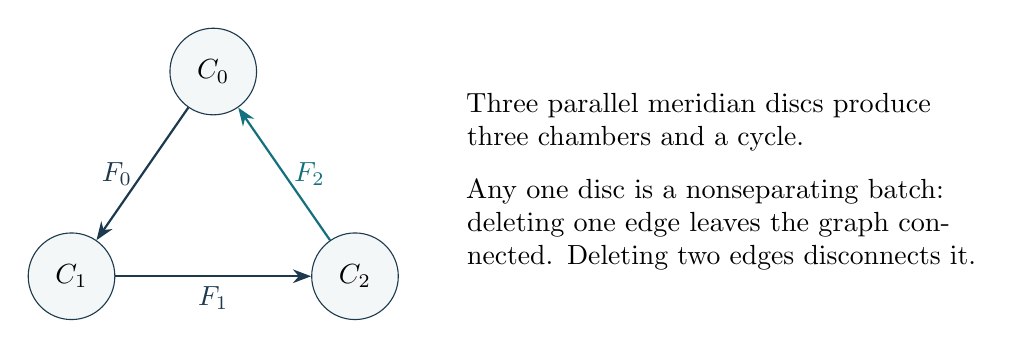
\begin{tikzpicture}[
 chamber/.style={circle,draw=ink,fill=pale,minimum size=11mm},
 every edge/.style={draw=ink,thick},
 >=Stealth]
\node[chamber] (a) at (0,1.8) {$C_0$};
\node[chamber] (b) at (-1.8,-0.8) {$C_1$};
\node[chamber] (c) at (1.8,-0.8) {$C_2$};
\draw[thick,->,ink] (a) -- node[left] {$F_0$} (b);
\draw[thick,->,ink] (b) -- node[below] {$F_1$} (c);
\draw[thick,->,accent] (c) -- node[right] {$F_2$} (a);
\node[align=left,text width=6.6cm,anchor=west] at (3.1,0.4)
 {Three parallel meridian discs produce three chambers and a cycle.\\[0.7em]
 Any one disc is a nonseparating batch: deleting one edge leaves the graph
 connected. Deleting two edges disconnects it.};
\end{tikzpicture}
\caption{A native stored example. Edge orientations choose component
coorientations and do not affect the connectivity criterion. The highlighted
edge is the complement of a spanning tree.}
\label{fig:three-meridians}
\end{figure}

\begin{proposition}[The chamber cycle obstruction, recalled]
\label{prop:cycle-obstruction}
For a connected orientable source and a disjoint system of connected
two-sided properly embedded surfaces,
\[
 \dim_{\Q}H_1(G;\Q)=k-|V(G)|+1
 \ \le\ \dim_{\Q}H_1(M;\Q).
\]
\end{proposition}
\begin{proof}
Choose a spanning tree of $G$. For every edge outside the tree, its edge
together with the tree path between its endpoints is a fundamental cycle;
loops are included. Realize the crossings of that cycle in small collars
of the corresponding surface components. Within each intervening chamber,
join consecutive collar endpoints by a path, using connectedness of the
chamber. The resulting closed curve in $M$ crosses the chosen non-tree
component once and crosses no other non-tree component.

Coorient the surfaces and orient each curve accordingly. Algebraic
intersection with the non-tree components defines linear functionals on
$H_1(M;\Q)$: the surfaces determine relative homology classes and their
boundaries lie in $\partial M$. On the constructed curves the matrix of
these functionals is the identity. Thus these curves have linearly
independent homology classes, one for each of the $k-|V(G)|+1$ non-tree
edges.
\end{proof}

This proof establishes existence of the paths. It supplies neither a
compressed path representation nor a source-support certificate for a
later edit. That distinction matters when using the graph in a hierarchy.
The obstruction itself is earlier mathematics from report~92.

\subsection{Independent verification and encoding costs}

The certificate \texttt{normal-chamber-graph-v1} contains the source
fingerprint, disc representatives, all marker addresses, the graph, and
three proof records: a weighted surface-label census, an unweighted
orientation-double count, and a weighted chamber-side census. Source changes
or changed normal coordinates invalidate the fingerprint.

The checker obtains the two chamber atoms from the independent raw cut-cell
reference~\cite{cutcells}, using its horizontal-face-to-chamber incidences. It derives the
surface marker from an independently reconstructed normal-arc recipe,
including the source edge orientation. It independently reconstructs chamber
pairings through the face-region reference, then replays all three orbit
proofs. It imports no exporter, chamber producer, graph decoder, or orbit
search. The validated finite source and the established normal-arc compiler
remain shared primitives, as in the maintained topology checkers.

Let $T$ be the tetrahedron count, $B$ the maximum normal-coordinate
bit length, and $k$ the explicit label count. The source incidence data
use $O(T\log(T+1))$ bits. Each orbit system has $O(T)$ interval
pairings with polynomially bounded endpoint bit lengths. Each marker query
starts with $O(k)$ runs. All marker weights are nonnegative and their total
mass is less than $2^{2k}$, so all transported scalars have $O(k)$ bits.
The graph has $k$ edges and at most $k+1$ vertices. Its incidence lists use
$O(k\log k)$ bits, while the current integer-mask and weight-run records
can require $O(k^2)$ bits. The complete construction and replay remain
polynomial in $T$, $B$, $k$, and the certificate trace lengths.

This is an output-sensitive assertion. A binary vector can describe
$N$ parallel discs, with $k=N$ exponential in the coordinate encoding.
Explicitly labelling all those components requires a correspondingly large
output. The operator does not hide this cost or silently quotient parallel
components. Incomplete component coverage is refused. In particular,
large-coordinate successful examples below are connected surfaces with
exponentially many discs, rather than exponentially many labelled components.

All three orbit queries share the caller's cycle allowance. An exhausted
allowance yields \texttt{INCONCLUSIVE} without a graph or certificate.
The checker can bound the combined number of recorded orbit events.
Neither limit is represented as a topological negative conclusion.

\subsection{An explicit native interface}

The supplied triangulation uses the maintained finite-source JSON schema;
normal coordinates are seven entries per tetrahedron in the established
four-triangle, three-quadrilateral order. Disc columns and ranks begin at
zero. A minimal use of the new API is:

\begin{lstlisting}[language=Python]
from fastunknot.normal_chamber_graph import normal_chamber_graph
from fastunknot.normal_chamber_graph_verify import verify_normal_chamber_graph

representatives = [{"tetrahedron": t, "column": c, "rank": r}]
result = normal_chamber_graph(
    triangulation, coordinates, representatives,
    record_certificate=True,
)
# Authenticate before consuming a successful graph:
if result["status"] == "COMPLETE":
    accepted = verify_normal_chamber_graph(
        triangulation, coordinates, result["certificate"]
    )
\end{lstlisting}

The complete call and checker signatures, including work bounds and
callback arguments, appear in the delivered source and reproduction
examples. The graph result is a new observer; it does not dispatch an
unknot verdict or replace the supplied-cut handlebody checker.


\section{Implementation audit and reproducible observations}
\label{sec:validation}

The mathematical statements above concern exact operations on specified
inputs. The experiments in this section check their relationship to the
delivered implementation. They also measure costs on complete public
queries, where source reconstruction, unchanged operations, and output
serialization can dominate the improved subroutine. The retained raw
records are the basis of every numerical table; the plotting script reads
those records directly.

\subsection{The changed trust boundary}

The old public weighted checker authenticates the source pairings and
weight intervals, verifies the unweighted AHT trace, reconstructs the
initial weight function, evaluates its transport, compares the final
histogram, and checks conservation. The new checker retains all these
steps and the same certificate schema. It changes the transport callback
to a local run-tree implementation.

The original flat transport remains executable as
\code{verify_weighted_orbit_certificate_reference}. The producer remains
separately implemented and does not import the new run tree. In particular,
the producer's quotient/remainder transport and the checker's
residue-anchor derivative are different arithmetic constructions of the
same push-forward. The separate weighted least-representative checker
also retains its earlier transport. Its forward weights and reverse
representative recovery are not silently replaced by histogram replay.

The chamber exporter introduces a new observer and certificate schema.
Its checker reconstructs marker addresses and chamber identifications
through the independent raw cut-cell reference described in
Section~\ref{sec:chambers}. Independence here means separate source
reconstruction and arithmetic paths at the stated interfaces. Both
checkers still rely on the established source validators, integer codec,
and unweighted orbit verifier. This is not a claim that every underlying
primitive has been independently reimplemented.

\subsection{Focused differential and adversarial tests}

The replay change passed 52 focused native test methods in a recorded
124.207-second run. These include the maintained moment-boundary test's
entire 157-source bank and full supplied-cut handlebody replay with
production paths disabled. Seven new test methods include:

\begin{itemize}
\item 500 random lazy range-add, split, and join transitions, checking the
full AVL height invariant, subtree lengths, endpoint values, and canonical
run sequence after every transition;
\item 1,000 random signed-vector translation folds, and every admitted
reflection fold, compared with literal point-fibre sums;
\item 400 random static deletions, with exact deleted histograms and the
remaining function compared with a literal reference;
\item interval lengths requiring more than 8,192 bits, without literal
expansion of the interval;
\item complete native star-family proofs accepted through both public
verifier variants, malformed-proof rejection, conservation checks, and
propagation of callback cancellation.
\end{itemize}

The eleven new chamber test methods independently exercise source labels,
two-sidedness, side markers, graph reconstruction, and subcuts. They include
nonzero triangle and quadrilateral ranks, signed edge identifications,
vertex and tetrahedron relabellings, representative reorderings, and an
actual reversal of the local coorientation. Multiple representatives on
one component are tested using distinct discs as invalid component labels.
Other cases cover omitted components, one-sided surfaces and their
connected two-sided doubles, empty surfaces, source and proof mutations,
hexadecimal integer encodings, booleans in integer fields, disabled
producers, shared work limits, and callback cancellation.

The maintained native suite was then run after the source files stabilized.
The broad run executed 1,733 methods in 499.532 seconds, with two failed
assertions and one class-setup error caused by a missing external fixture.
After restoring the exact pinned fixture, all eight methods in that class
passed. Thus the completed audit exercised all 1,741 declared methods.
The exact logs are \code{results/full_native_suite.log} and
\code{results/transport_annulus_fixture_rerun.log}.

Both failed assertions were independently reproduced in fresh workers using
the exact pinned source and in workers using the lazy patch: each expected
\code{INCONCLUSIVE} but received \code{COMPLETE}. They occur in
\code{test_core_primitive_annuli.py} and
\code{test_disk_bundle_absorption.py}; the pinned adaptive lower-forest
tests explicitly require the successful outcomes on those same sources.
The source-authenticated baseline audit retains the identical tracebacks
and hashes in \code{results/baseline_failure_audit.json}. These two stale
expectations remain unchanged. No additional source failure was observed.

An earlier verbose attempt was interrupted during a filesystem-capacity
incident; its partial log is retained separately and is not counted as
completed regression evidence. The restored-fixture run described above
resolves the environmental setup error. These are executed finite
regression and differential checks, not a proof-assistant formalization
of the article's theorems.

\subsection{Complete weighted-certificate measurements}

Table~\ref{tab:star-timing} measures the entire public weighted-certificate
verification call for the star family. It includes source weight
validation, initial canonicalization, independent authentication of the
unweighted trace, and final histogram checks. Certificate generation is
recorded separately and is outside this timed interval.
Each row contains three paired repetitions. The figure shows all samples
and the median for each backend.

\begin{table}[htbp]
\centering\small
\begin{tabular}{rrrrr}
\toprule
$H$ & $L$ & Flat (s) & Lazy (s) & Ratio \\
\midrule
16 & 256 & 0.008291 & 0.002036 & 4.073$\times$ \\
32 & 1,024 & 0.075450 & 0.007252 & 10.404$\times$ \\
64 & 4,096 & 0.602308 & 0.030957 & 19.456$\times$ \\
128 & 16,384 & 4.745231 & 0.121760 & 38.972$\times$ \\
\bottomrule
\end{tabular}

\caption{Median complete weighted verification times on the legal star
family. A ratio greater than one means the lazy variant was faster.
Here \(L=H^2\); all displayed widths are even.}
\label{tab:star-timing}
\end{table}

\begin{figure}[htbp]
\centering
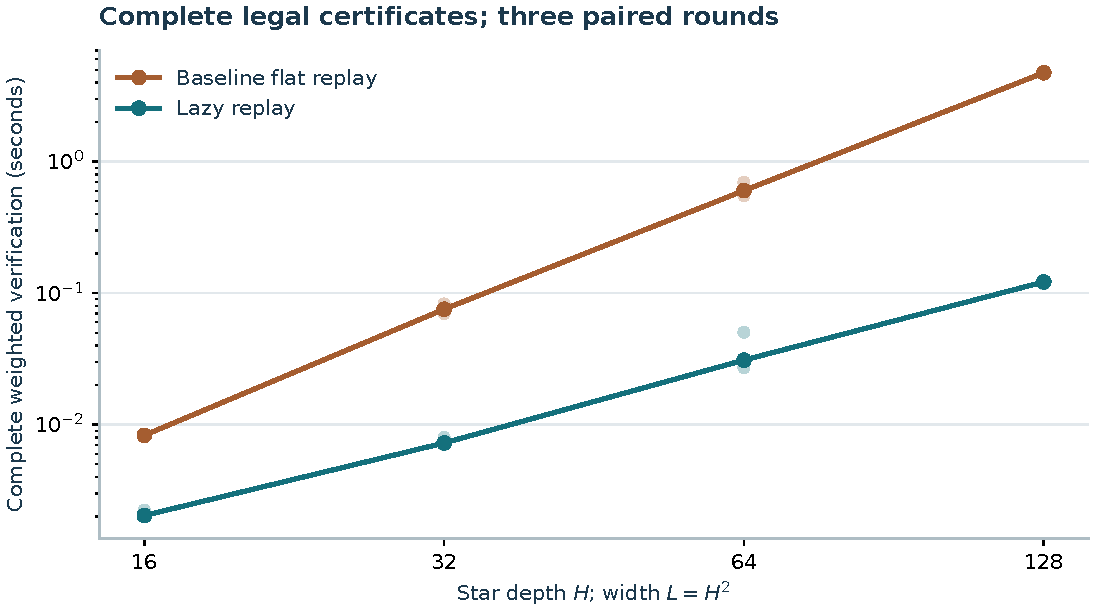
\includegraphics[width=0.93\textwidth]{figures/synthetic_replay.pdf}
\caption{Observed complete weighted replay on one machine. The pale
points are the three individual measurements; connected points are
medians. The proof of Theorem~\ref{thm:star}, rather than a fitted timing
curve, establishes the asymptotic separation.}
\label{fig:star-timing}
\end{figure}

At \(H=128\), the initial state has 16,384 runs. The complete native trace
contains 128 truncations and one contraction. The instrumentation records
128 removed suffix runs in total, 255 range additions, and 16,384 emitted
runs. Reading a receiving subtree's stored run count records over two
million receiver-run incidences without visiting those leaves. The final
histogram has precisely two entries, weights 128 and 129, each with
multiplicity 8,192. These counters connect the measured example to the
mechanism in the proof.

The implementation was measured under Python 3.12.14 on a Linux x86-64
environment. The full interpreter and platform strings are stored with
the data. Three repetitions on one shared host do not establish a
hardware-independent speed factor or a statistical confidence interval.
The source family demonstrates a legal orbit-trace obstruction to eager
replay; no claim is made that these orbit systems are a family of hard
knot-complement normal cuts.

\subsection{Paired native supplied-cut queries}

The native benchmark uses eleven source/method pairs: eight maintained
case/method choices and three genuine layered-solid-torus meridians with
coordinates multiplied by three. It includes both moment and mask boundary
methods. Raw triangulations and coordinates are bundled, so replay needs
no fixture generator or Regina installation.

The old and new verifiers run in isolated Python processes. The baseline
package is restored using the exact pinned verifier bytes; no module-binding
monkeypatch substitutes an old implementation at runtime. In each of three
paired rounds, the benchmark freshly reconstructs the source, produces a
complete supplied-cut certificate, runs public whole-cut verification, and
serializes the result as canonical JSON. Every certificate was independently
accepted and every complete-result digest agreed between the variants.
Source preparation is included in the relevant production and verification
calls, rather than reported as an omitted preprocessing step.

\begin{table}[htbp]
\centering\footnotesize
\setlength{\tabcolsep}{4pt}
\begin{tabular}{lrrrr}
\toprule
Source/method & Flat replay & Lazy replay & Replay ratio & Query ratio \\
\midrule
Pilot LST, moments & 0.0141 & 0.0139 & 1.011 & 1.004 \\
Pilot trefoil, moments & 0.0038 & 0.0038 & 0.992 & 1.004 \\
Solid torus/RP3, moments & 0.0119 & 0.0126 & 0.942 & 0.948 \\
Interior mixed, moments & 0.0656 & 0.0483 & 1.360 & 1.169 \\
Fibonacci 09 mixed, moments & 0.7988 & 0.5812 & 1.374 & 1.134 \\
Trefoil mixed, moments & 0.1302 & 0.1109 & 1.174 & 1.111 \\
Pilot LST, masks & 0.0178 & 0.0150 & 1.186 & 1.123 \\
Interior mixed, masks & 0.0618 & 0.0517 & 1.195 & 1.271 \\
Layered meridian $T=4$ & 0.2043 & 0.1510 & 1.353 & 1.122 \\
Layered meridian $T=8$ & 0.8797 & 0.7274 & 1.209 & 1.087 \\
Layered meridian $T=16$ & 3.9349 & 3.4831 & 1.130 & 0.925 \\
\midrule
Sum of case medians & 6.1229 & 5.1989 & 1.178 & 0.982 \\
\bottomrule
\end{tabular}

\caption{All native paired results. Replay times are seconds; ratios
are baseline/new medians. The query ratio includes production, whole-cut
verification, and serialization. The layered rows use moments and scale
three. The final row is a ratio of sums of case medians.}
\label{tab:native-timing}
\end{table}

The sum of case-median replay times decreased from 6.122913 to 5.198893
seconds, a ratio of \(1.1777\). The corresponding complete-query totals
were 14.109865 and 14.364058 seconds: the new run was approximately
\emph{1.8 percent slower}. The data therefore support an aggregate replay
improvement but do not support an aggregate complete-query speed-up.

The largest discrepancy occurred in the \(T=16\) layered case. Its unchanged
producer took median 5.253965 seconds in the baseline worker and 6.811022
seconds in the new worker, while whole-cut verification improved from
3.934936 to 3.483064 seconds. The producer source is identical between
variants. These measurements alone do not establish the cause of its
time variation. The original samples, including the unfavorable aggregate
and the small-case regression, are retained without replacement.

The timing scope is a supplied normal-cut handlebody census, not a
diagram-to-verdict unknot run. It is also broader than the changed ordinary
weighted replay: two representative-selector queries and other source
work remain unchanged. These facts explain why the synthetic verifier
ratios cannot be multiplied into a claimed recognition speed factor.
A controlled repetition addressing the producer variation is a useful
future experiment; it is not a reason to discard the present observation.

\subsection{Geometric chamber checks on native inputs}

The maintained corpus contains 106 inputs. Among 99 inputs small enough
for the deliberately bounded literal reference, 80 produced independently
accepted chamber graphs and 19 were correctly refused because their
surfaces contain a one-sided component. The seven remaining binary
multiplicity cases correctly refused an incomplete representative list.
An inconclusive response on those inputs is a source-contract outcome,
not a negative topological verdict.

For all accepted small inputs, 254 exhaustive labelled subbatch checks
agreed with \emph{two} independent literal constructions. The first
reglues every actual normal-disc face of each omitted component into the
full cut. The second forms the normal vector of exactly the selected
components, independently regenerates that subcut, and counts its
literal chamber components. The components themselves are identified by
gluing individual face-arc disc ranks, rather than by reusing the native
normal-edge orbit census. These checks cover separating bridges,
one-vertex loops, mixed systems, and the three-cycle in
Figure~\ref{fig:three-meridians}.

Large-coordinate connected meridians were checked separately.
Table~\ref{tab:chamber-stress} records single feasibility samples, without
a baseline or comparative speed claim.

\begin{table}[htbp]
\centering\small
\setlength{\tabcolsep}{4pt}
\begin{tabular}{rrrrrr}
\toprule
$T$ & Coordinate bits & Orbit cycles & Proof bytes & Produce (s) & Replay (s) \\
\midrule
16 & 11 & 110 & 147,835 & 0.0167 & 0.0125 \\
32 & 22 & 206 & 555,642 & 0.0613 & 0.0311 \\
64 & 44 & 398 & 2,165,507 & 0.2722 & 0.0991 \\
128 & 89 & 782 & 8,538,169 & 1.1494 & 0.3594 \\
\bottomrule
\end{tabular}

\caption{Connected meridians of Fibonacci layered solid tori.
Proof size is compact uncompressed JSON bytes. Each graph consists of
one vertex and one loop.}
\label{tab:chamber-stress}
\end{table}

The \(128\)-tetrahedron example has exactly
\[
2\,791\,715\,456\,571\,051\,233\,611\,642\,548
\]
normal discs, maximum coordinate bit length 89, and one component. A
representative at a large nonzero quadrilateral rank authenticates its
one-loop graph. The certificate has 8,538,169 bytes and the three queries
use 782 orbit cycles. The corresponding single observed production and
replay times were 1.149 and 0.359 seconds.

These connected examples use the maintained single-orbit shortcut in the
weighted queries. They demonstrate that native graph authentication can
handle enormous literal disc counts at small component count; they are
not a separate benchmark of the new lazy fold. The complete small
three-meridian packet and the \(128\)-tetrahedron packet are retained so
that their source validation and graph replay can be repeated directly.

\section{Consequences for the hierarchy program and further research}
\label{sec:global}

The results improve two specific entries in the complexity ledger:
weighted certificate evaluation and authentication of a graph interface.
They do not reduce the number of candidate surfaces considered, justify an
arbitrary reordering of a hierarchy, or bound how many times an earlier
surface can invalidate later work. It is useful to state these distinctions
as mathematical dependencies rather than as a single undifferentiated
claim of progress.

\subsection{The remaining global budget}

Let \(\Sigma\) be the set of actually visited geometric states, counting
revisits that require new work. A useful implementation ledger is
\[
 T_{\rm total}\ \le\
 \sum_{\sigma\in\Sigma}
 \left(C_{\rm source}(\sigma)+C_{\rm search}(\sigma)
       +C_{\rm edit}(\sigma)+C_{\rm verify}(\sigma)
       +C_{\rm output}(\sigma)\right).
\]
Every term must be evaluated in encoded size: source records, coordinate
bits, pattern labels, certificate events, and output records. The lazy
ledger improves a term inside \(C_{\rm verify}\). The chamber observer
supplies a checked predicate that may eventually help control
\(\Sigma\), once its geometric witnesses can be transported.

If the number of visited states were at most \(n^{a\log n}\) and every
state's total encoded work at most \(n^b\), then the displayed sum would
be \(n^{a\log n+b}\). That elementary multiplication explains what would
be sufficient for the announced target, but neither hypothesis follows
from a polynomial orbit primitive. In particular, a polynomially bounded
hierarchy length does not by itself bound the number of discarded and
rebuilt suffixes.

The restart estimate \(L(g+1)^L\) in the cited hierarchy discussion is
especially informative here. For \(g\le n^a\) and \(L\le cn\), it
only yields \(n^{O(n)}=\exp(O(n\log n))\); it does not yield
\(n^{O(\log n)}\). A logarithmic effective dependency depth, or another
proved reuse or search mechanism of comparable strength, would need to
replace that accounting for this implementation. Earlier repository
reports already establish abstract dependency and weighted reset
bounds~\cite{repair,persistence}. The unresolved issue is to authenticate
their hypotheses through actual geometric operations, rather than
state the abstract recurrence again.

\subsection{A source-to-graph complexity statement}

\begin{corollary}[Encoded native chamber query]
\label{cor:encoded-chamber}
Let the validated triangulation have \(t\) tetrahedra and the maximum
coordinate bit length be \(B\). Let the supplied representative list have
length \(k\). Subject to the established encoded bounds for the native
normal arc and chamber interval systems and a polynomial AHT schedule,
the complete chamber query and verification of its produced certificate
have polynomial cost in \(t+B+k\), including all three orbit queries and
the binary source data. Verification of an arbitrary supplied trace also
charges that trace's encoded length. The graph has \(k\) edges and at
most \(k+1\) vertices. For nonnegative additive component rewards, it
supports a maximum-reward simultaneously nonseparating subbatch by a
minimum spanning tree of the authenticated graph.
\end{corollary}
\begin{proof}
The local interval systems have a number of records polynomial in \(t\)
and endpoints with \(O(B+\log(t+1))\) bits. The first and third queries add
at most \(k\) and \(2k\) singleton intervals with marker values of at most
\(k\) and \(2k\) bits respectively. Doubling adds one bit to the relevant
coordinates. Apply the encoded weighted-orbit bounds to these actual
systems and include their checked traces. The lazy implementation has
polynomial run, value, and output bounds and the finer ledger of
Corollary~\ref{cor:lazy-replay}. The graph construction and its independent
verification are polynomial in \(k\). The vertex bound and the spanning-tree
optimization follow from Theorem~\ref{thm:native-chamber} and
Corollary~\ref{cor:batch-optimizer}.
\end{proof}

This statement is polynomial in the \emph{explicit} representative count.
For \(m\) parallel meridian discs of a solid torus, the graph is a cycle
with \(m\) edges, with a loop when \(m=1\) and two parallel edges when
\(m=2\). An explicit output takes \(\Omega(m)\) records although the normal
vector uses only \(O(\log m)\) multiplicity bits. This family explains
exactly why the parameter \(k\) cannot be deleted from the corollary.

\subsection{What has and has not become reusable}

Before this continuation, report~92's graph decoder could authenticate a
finite scalar partition relative to a supplied source relation and side
markers. It could not derive all of those inputs from the native normal
vector. The new exporter supplies that missing step for labelled components
of one normal surface. This turns an abstract input contract into an
executable source-bound observer.

There are still two distinct geometric gaps. First, a path in a chamber
graph lifts to a path in the manifold by connectedness, but that existence
argument does not produce a compressed, source-addressed path. Second, an
edit can leave the graph numerically unchanged while altering the embedded
surfaces, boundary marking, or the predicates needed by the hierarchy.
Neither unchanged graph data nor a reused orbit trace proves that a
certificate survives such an edit.

For actual persistent hierarchy work, a certificate should eventually
include the surface, its side data, a geometric dual route, and the
source records read in validating all relevant predicates. Only then can
an edit be checked against the certificate's geometric dependencies.
Reports~92 and~98 already identify this distinction
\cite{persistence,gauge}. The present exporter advances the source
authentication layer; it does not skip the route or edit layers.

\Needspace{9\baselineskip}
\subsection{The initial knot-exterior limitation}

\begin{proposition}[No large first nonseparating batch]
\label{prop:rank-one}
In a knot exterior in \(S^3\), a system of disjoint compact connected
two-sided properly embedded surfaces whose simultaneous cut complement
is connected has at most one member.
\end{proposition}
\begin{proof}
The chamber-cycle argument in Section~\ref{sec:chambers} provides, for
such a system of \(j\) surfaces, \(j\) independent integral intersection
functionals on \(H_1(M;\Z)\). A knot exterior has
\(H_1(M;\Z)\cong\Z\), so \(j\le1\). Equivalently, the graph cycle rank
cannot exceed the first Betti number.
\end{proof}

This is the earlier obstruction from report~92, included here because it
applies directly to the new API. It rules out a proposed algorithm that
obtains a large initial parallel batch merely by asking this observer for
many disjoint nonseparating components. It does not bound sequential
hierarchy length. Later surfaces live in later cut pieces and need not
coembed as a disjoint system in the original exterior.

\subsection{A useful next replay theorem}

Lazy addition is favorable when the receiver is complicated and the
transported addition is simple. A dense reflection can instead have
\(S\) comparable with \(R\), in which case a flat linear sweep can be
cheaper than \(S\) separate logarithmic updates.

\begin{proposition}[A cost-controlled hybrid, not implemented here]
\label{prop:hybrid}
Suppose both the lazy evaluator and an eager linear merge of the old
weight function with the canonical transported addition are available.
The stored total and suffix run counts permit a choice, before either
receiver is expanded, with structural cost
\[
 O\!\left(
 S\log(S+1)+
 \min\{R,(S+1)\log(R+2)\}
 \right)
\]
for a translation fold, and with no sorting term for reflection.
Corresponding vector arithmetic and binary costs must also be included.
\end{proposition}
\begin{proof}
The lazy option is Theorem~\ref{thm:lazy-fold}. The eager option
materializes the current tree, reports the suffix, constructs the
transported addition, merges the two ordered partitions, and rebuilds a
balanced tree. Excluding the translation's common residue sorting term,
this costs \(O(R+S)=O(R)\), since \(S\le R\). A suffix count is obtained
from an \(O(\log R)\) split, and the total count is stored at the root.
Select the cheaper upper bound. The selection overhead is dominated by
the displayed bound. Both options compute the same exact canonical
function, so the choice changes cost only.
\end{proof}

The proposition is a proved design option, not a statement that the
delivered implementation already chooses between those two whole-state
strategies. The measured code uses the lazy replay method and retains the
old complete flat verifier as an explicit reference. Any production
threshold should be tested against actual source distributions, including
small cases and dense reflection cases.

\subsection{Research questions with concrete next deliverables}

\begin{enumerate}[leftmargin=*,label=\textbf{\arabic*.}]
\item \textbf{Lazy representative transversals.}
The ordinary histogram verifier now avoids repeated receiver scans, but
the separate least-representative verifier retains its older forward
weights and reverse gap-insertion procedure. Can a labelled order
structure achieve comparable bounds while preserving the \emph{least
original representative}, not merely the correct histogram? A useful
deliverable is a replay engine with an independent label oracle and a
full-query benchmark.

\item \textbf{Ordered batch range additions.}
Can all \(S\) consecutive addition intervals be applied by one joint
tree traversal in
\(O(S\log(1+R/S)+S)\) structural work? Any proof must include
canonical seam merging, lazy-tag propagation, and the cost of creating
and discarding temporary boundaries. This could improve the dense
regime without flattening the entire state.

\item \textbf{A measured hybrid policy.}
Implement Proposition~\ref{prop:hybrid}, or a simpler justified
threshold, and test whether small-case overhead or dense reflections
warrant the extra branch. Compare complete replay, not just isolated
tree updates.

\item \textbf{Histogram aggregation with a strict comparison bound.}
The delivered evaluator uses Python dictionaries for emitted vectors,
as does the established checker. A sorted emission ledger or an
ordered map would make the fine comparison bound independent of hash
behavior. Determine whether that choice is helpful at the dimensions
and vector sizes actually produced by the geometry.

\item \textbf{A separate lazy producer.}
The producer retains quotient/remainder transport while the verifier
uses a residue derivative. Apply receiver-independent storage to
production with a separately written transport path, and measure
whether generation becomes the next bottleneck. Sharing the same
arithmetic between both sides would weaken the present differential
check.

\item \textbf{Integration with static endpoint contraction.}
The incoming exceptional-row package changes other replay costs,
including pairing endpoint contraction and source reuse. Combine the
patches at one source revision and measure their interaction. Ratios
from different baselines must not be multiplied to manufacture a
combined speed-up.

\item \textbf{Automatic component representatives.}
The native graph API validates representatives; it does not discover a
short exhaustive list for an arbitrary normal vector. Can least
representative intervals be converted to normal-disc addresses
without enumerating components that occur in large parallel
multiplicity? State the unavoidable output dependence explicitly.

\item \textbf{A graph grammar for parallel families.}
Replace the explicit \(k\)-edge output by a source-certified grammar
when many components have repeated chamber incidence. The cycle
family of parallel meridians supplies a basic binary test. Report~98's
graph operators can be used only after the grammar's geometric
interpretation has been authenticated.

\item \textbf{Geometric dual-route extraction.}
Given an accepted graph and a spanning tree of the undeleted edges,
construct a route in actual source charts crossing a selected
component once. The route should remain short in encoded size even
when its literal length is large, and its verifier should reconstruct
all endpoint identifications.

\item \textbf{Persistence through a real local edit.}
Apply one genuine source edit, transport the component and dual-route
certificates, and prove precisely which read records remain valid.
This is the next needed connection to the causal-restart theory,
rather than another abstract dependency bound.

\item \textbf{Broader finite boundary contracts.}
The current source validator admits one torus boundary. Later hierarchy
pieces can have many boundary components and corners or patterns.
Extend the validator and the side-marker construction to that setting
without treating boundary Euler characteristic as a substitute for
the full manifold-link checks.

\item \textbf{Marked-boundary transport.}
The graph records sides of the supplied surfaces, not all later
boundary-pattern arcs. Determine which additional labels are
sufficient to preserve the hierarchy predicates, and bound their
growth under cut, compression, and normalization.

\item \textbf{Measure actual dependency depth.}
Once the preceding geometric operations exist, instrument genuine
certificate invalidations. Test whether the validated dependency depth
is logarithmic, and whether counter ranges and version changes obey
the already proved reset models. Disjoint surface supports alone are
insufficient evidence.

\item \textbf{Joint source, trace, and state bounds.}
Give one recurrence in the original crossing number that bounds
source size, coordinate and pattern bits, generated candidates,
all orbit traces, and all restarts. A polynomial local primitive
becomes part of a quasi-polynomial recognizer only after this joint
accounting is established.
\end{enumerate}

The immediate implementable priorities are labelled transversal replay,
automatic representative addresses, and one source-authenticated dual
route. The next substantial geometric milestone is persistence of that
route and all required predicates through an actual hierarchy edit.

\section{Delivered artifacts and integration}
\label{sec:integration}

The archive is intended to be reviewable before integration into the
repository. It contains the article source and PDF, the changed native
modules and tests, a patch against the pinned source, a small runnable
snapshot with the required unchanged dependencies, the original verifier,
raw source packets, exact observed results, and reproduction programs.
The source checkpoint is \BaseCommit.

\subsection{Native changes}

All six changed or new repository files are under
\code{Topology/UnknotRecognition/fast/}. The files are:

\begingroup\small
\begin{longtable}{L{0.46\textwidth}L{0.46\textwidth}}
\toprule
Path below the native fast directory & Purpose\\
\midrule
\endhead
\code{fastunknot/weighted_run_rope.py} &
New deterministic AVL run sequence and local weight transport.\\
\addlinespace
\code{fastunknot/weighted_orbit_verify.py} &
Select lazy transport in ordinary histogram replay and retain the
explicit original reference verifier.\\
\addlinespace
\code{fastunknot/normal_chamber_graph.py} &
New source-derived component-label, side-marker, and chamber-graph
producer.\\
\addlinespace
\code{fastunknot/normal_chamber_graph_verify.py} &
New independently reconstructed chamber-graph checker.\\
\addlinespace
\code{tests/test_weighted_run_rope.py} &
Literal arithmetic oracles, structural invariants, legal-trace
separation, and invalid-proof checks.\\
\addlinespace
\code{tests/test_normal_chamber_graph.py} &
Literal component/subcut references, source-bound graph checks,
encoding, relabelling, and resource-limit tests.\\
\bottomrule
\end{longtable}
\endgroup

The chamber observer adds the schema
\code{normal-chamber-graph-v1}. Existing weighted-orbit and supplied-cut
certificate schemas are unchanged. The integration does not modify the
diagram recognizer's verdict dispatch. Successful chamber export and
successful supplied-cut certification remain their respective local
geometric conclusions.

\subsection{Package layout and provenance}

\begin{longtable}{L{0.42\textwidth}L{0.50\textwidth}}
\toprule
Archive location & Content\\
\midrule
\endhead
\code{article/} &
Main \LaTeX\ source, section files, bibliography, generated tables,
vector figure, and compiled PDF.\\
\addlinespace
\code{integration/overlay/} &
Only the six modified/new files, at their repository-relative paths.\\
\addlinespace
\code{integration/proveit_lazy_replay_chamber_graphs.patch} &
Unified patch against the pinned repository.\\
\addlinespace
\code{integration/native_snapshot/} &
Runnable package and the fixture/test dependency closure needed for the
new checks; it is not a second full repository.\\
\addlinespace
\code{integration/reference/} &
Exact original weighted verifier used for baseline comparison.\\
\addlinespace
\code{results/} &
Original paired timing samples, complete-suite and focused logs,
native audit records, and source fixture records.\\
\addlinespace
\code{examples/} &
Complete three-meridian and large connected-meridian source/certificate
packets.\\
\addlinespace
\code{scripts/} &
Portable benchmark, chamber audit, stored-packet replay, and figure
generation programs.\\
\addlinespace
\code{reproduce.py} &
A small command-line entry point for the bundled checks and optional
benchmark reproduction.\\
\bottomrule
\end{longtable}

The recorded benchmark source and the later portability adaptation are
both retained. The portability adaptation adds explicit package,
fixture, and baseline-verifier paths; it does not alter the timed worker
body or the measured native implementation. Source hashes identify the
baseline and measured files. The archive manifest identifies its
delivered files, and the integration provenance records the source pin.

\subsection{Reproduction without external services}

From the unzipped archive root, the bundled checks are:

\begin{lstlisting}
python reproduce.py
\end{lstlisting}

This runs the eighteen new test methods and verifies the two complete
stored chamber packets. It needs Python 3.10 or newer and the bundled
standard-library-based native source. It does not need a network
connection, a Git checkout, Regina, or an external topology service.
Use the following optional modes to repeat the original scope of the
measurements and the complete chamber audit:

\begin{lstlisting}
python reproduce.py --synthetic
python reproduce.py --native
python reproduce.py --chamber-audit
\end{lstlisting}

New results are written under \code{reproduced/}; the original observations
under \code{results/} remain the evidence reported in this article.
The native comparison includes one warmup per case and backend,
alternates variant order, and checks every result digest. The synthetic
comparison times whole weighted verification and reports generation
separately. Wall-clock measurements will vary across machines.

The article can be rebuilt from \code{article/} with:

\begin{lstlisting}
latexmk -pdf -interaction=nonstopmode \
  -halt-on-error Lazy_Replay_and_Native_Chamber_Graphs.tex
\end{lstlisting}

A conventional \LaTeX\ installation with the packages named in the main
source is sufficient; the already generated vector figure is included.
Regenerating that figure and the numerical tables additionally needs
Matplotlib and runs \texttt{python} \code{scripts/make_figures.py} from the archive
root. It reads the original JSON records and does not rerun timings.

\subsection{Applying the source changes}

In a review checkout at the pinned revision, the patch can be checked
and applied with:

\begin{lstlisting}
git apply --check /path/to/archive/integration/\
proveit_lazy_replay_chamber_graphs.patch
git apply /path/to/archive/integration/\
proveit_lazy_replay_chamber_graphs.patch
\end{lstlisting}

The package includes an applicability check against clean pinned source
files. If later repository changes overlap these paths, they require
ordinary source review and a fresh regression run. In particular, the
incoming source-reuse and endpoint-contraction patches concern adjacent
costs and have not been silently incorporated into the measured baseline.

For the full maintained suite in an integrated checkout, run from
\code{Topology/UnknotRecognition/fast/}:

\begin{lstlisting}
python -B -m unittest discover -s tests
\end{lstlisting}

The recorded full-suite command uses the actual maintained checkout.
The compact snapshot is intended for the new tests, packet replay, and
included benchmarks; it does not claim to reproduce every unrelated
maintained test without the rest of the repository.

\Needspace{10\baselineskip}
\subsection{Claim and evidence ledger}

\begin{longtable}{L{0.30\textwidth}L{0.34\textwidth}L{0.28\textwidth}}
\toprule
Claim & Basis & Limit\\
\midrule
\endhead
Receiver-independent fold cost &
Exact lazy-action, balanced-tree, and residue proofs &
Integer, histogram, and unweighted-trace costs are explicit separate terms.\\
\addlinespace
Asymptotic replay separation &
Arbitrary-parameter legal star family &
Comparison with the specified eager method; no hard-knot family asserted.\\
\addlinespace
Native chamber graph correctness &
Component-label census, normal double, side census, independent charts &
Supplied admissible surface, explicit representatives, current source domain.\\
\addlinespace
All labelled subcut partitions &
Regluing theorem and graph connectivity &
Nonseparation does not prove incompressibility or handlebody structure.\\
\addlinespace
Observed replay improvements &
All retained paired samples and exact accepted result digests &
The aggregate native complete-query time regressed in this run.\\
\addlinespace
Large-coordinate feasibility &
Complete native \(128\)-tetrahedron packet &
One component; single-orbit shortcut; no expanded graph with exponentially
many labelled edges.\\
\addlinespace
General quasi-polynomial recognition &
Research target and explicit outstanding dependencies &
Not proved or implemented by this continuation.\\
\bottomrule
\end{longtable}

The next source-level milestone is a compressed geometric dual route whose
complete validation dependencies survive one actual hierarchy edit.
The new observer supplies component and side identities for that work.
The new replay method reduces an already measurable cost of checking the
resulting local certificates.

\begin{thebibliography}{99}
\raggedright
\bibitem{aht}
Ian Agol, Joel Hass, and William Thurston,
\emph{The computational complexity of knot genus and spanning area},
Transactions of the American Mathematical Society \textbf{358} (2006),
3821--3850.
\url{https://arxiv.org/abs/math/0205057}.

\bibitem{announcement}
University of Oxford Mathematical Institute,
\emph{Marc Lackenby announces a new unknot recognition algorithm that runs
in quasi-polynomial time}, 2 February 2021.
\url{https://www.maths.ox.ac.uk/node/38304}.

\bibitem{talk}
Marc Lackenby,
\emph{Unknot recognition in quasi-polynomial time},
lecture slides, February 2021.
\url{https://people.maths.ox.ac.uk/lackenby/quasipolynomial-talk.pdf}.
The slides are referenced, not redistributed.

\bibitem{lackenby26}
Marc Lackenby,
\emph{Incompressible surfaces, hierarchies and unknot recognition},
arXiv:2607.23350v1, 25 July 2026.
\url{https://arxiv.org/abs/2607.23350v1}.

\bibitem{repo}
Vladimir Reshetnikov and ProveIt contributors,
\emph{ProveIt: Topology/UnknotRecognition},
source revision \BaseCommit, inspected 12 October 2026.
\url{https://github.com/VladimirReshetnikov/ProveIt/tree/e0b2f802f336fcb51e9ec5f29174cfe28dfb9d39/Topology/UnknotRecognition}.

\bibitem{suffix}
ProveIt contributors,
\emph{A sharp bound and local arithmetic for suffix weight folds},
maintained synthesis chapter \code{suffix_folds.tex}, same pinned revision.
\url{https://github.com/VladimirReshetnikov/ProveIt/blob/e0b2f802f336fcb51e9ec5f29174cfe28dfb9d39/Topology/UnknotRecognition/synthesis/suffix_folds.tex}.

\bibitem{weighted}
ProveIt contributors,
\emph{Native weighted normal components and essential-disc counts},
maintained synthesis chapter \code{weighted_components.tex}, same revision.
\url{https://github.com/VladimirReshetnikov/ProveIt/blob/e0b2f802f336fcb51e9ec5f29174cfe28dfb9d39/Topology/UnknotRecognition/synthesis/weighted_components.tex}.

\bibitem{persistence}
ProveIt contributors,
\emph{Cographic Persistence and Causal Reset Complexity for Compressed
Unknot Hierarchies}, report~92, 12 October 2026.
\url{https://github.com/VladimirReshetnikov/ProveIt/blob/e0b2f802f336fcb51e9ec5f29174cfe28dfb9d39/Topology/UnknotRecognition/reports/92/article/cographic_persistence_standalone.tex}.

\bibitem{repair}
ProveIt contributors,
\emph{Exact symbolic compression for unknot recognition:
graded transfer, finite twist tails, and the remaining complexity barrier},
report~23, \code{unknot_symbolic_compression.tex}, same pinned revision.
\url{https://github.com/VladimirReshetnikov/ProveIt/blob/e0b2f802f336fcb51e9ec5f29174cfe28dfb9d39/Topology/UnknotRecognition/reports/23/article/unknot_symbolic_compression.tex}.

\bibitem{gauge}
ProveIt contributors,
\emph{Component-Gauge Cut Atlases for Compressed Unknot Hierarchies},
report~98, same pinned revision.
\url{https://github.com/VladimirReshetnikov/ProveIt/blob/e0b2f802f336fcb51e9ec5f29174cfe28dfb9d39/Topology/UnknotRecognition/reports/98/article/component_gauge_atlases.tex}.

\bibitem{cutcells}
ProveIt contributors,
\emph{Full compressed normal-cut cells and reconstruction charts},
native modules \code{normal_cut_cells.py} and
\code{normal_cut_cells_verify.py}, same pinned revision.
\url{https://github.com/VladimirReshetnikov/ProveIt/tree/e0b2f802f336fcb51e9ec5f29174cfe28dfb9d39/Topology/UnknotRecognition/fast/fastunknot}.

\end{thebibliography}

\end{document}
